\documentclass[aspectratio=169]{beamer}
\usepackage{graphicx}
\usepackage{stmaryrd}
\usepackage[T1,T2A]{fontenc}
\usepackage[utf8]{inputenc}
\usepackage[english,russian]{babel}
\usepackage{amsmath}
\usepackage{amsfonts}
\usepackage{amssymb}
\usepackage{makeidx}
\usepackage{verbatim}
\usepackage{amsthm}
%\usepackage{bnf}
\usepackage{tikz}
\usepackage{enumerate}
\usepackage{mathtext}
\usepackage{mathtools}
\usepackage{mathabx}
%\usepackage[left=2cm,right=2cm,top=2cm,bottom=2cm,bindingoffset=0cm]{geometry}
\usepackage{proof}
%\usepackage{paracol}
%\usepackage{enumitem}
\usepackage{color}
\usepackage{colortbl}
\usepackage{multicol}
%\usepackage{minted}
%\usepackage{hyperref}
\setbeamertemplate{navigation symbols}{}
\usetikzlibrary{graphs}
\usetikzlibrary{graphs.standard}
\usetikzlibrary{automata,positioning}
\usepackage{float}

\begin{document}

%\theoremstyle{dfn}
\newtheorem{dfn}{Определение}[section]
\newtheorem{nte}{Замечание}[section]

\newtheorem{axiom}{Аксиома}[section]
\newtheorem{thm}{Теорема}[section]
\newtheorem{lmm}[theorem]{Лемма}
\newtheorem{statement}{Утверждение}[section]
\newtheorem{oun_paragraph}{Пункт}[section]
\newtheorem{cons}{Следствие}[section]
\newtheorem*{exm}{Пример}

\newcommand{\comb}[1]{\operatorname{\mathcal{#1}}}
\newcommand{\func}[1]{\operatorname{#1}}
\newcommand{\reduction}[1]{{\color{OrangeRed}#1}}
\newcommand{\set}[1]{\left\{#1\right\}}

\def\from#1{\par \parbox{0.7\textwidth}{\par \hfill\raggedleft \it #1}} 

\begin{frame}{}
\begin{center}
{\LARGE Теория типов}\\\vspace{1cm}
\large О курсе
\end{center}
\end{frame}

\begin{frame}{Краткое содержание вступительного занятия}
\begin{enumerate}
\item История вопроса: что вообще изучает теория типов, типы в математике, типы в лямбда-исчислении.
Краткое повторение материала, знание которого ожидается от участников.
\item Содержание текущего курса: изоморфизм Карри-Ховарда и его применение в программировании и математике
\item Особенности преподавания.
\end{enumerate}
\end{frame}

\begin{frame}{Типы в теории множеств}
\begin{itemize}
\item Парадокс Рассела: $\{\ x\ |\ x \notin x\ \}$. Законна ли эта запись?
$a \in b$ --- ожидаем, что слева элемент, а справа множество. %Интуитивно хочется такие ситуации запретить.

\item Давайте запретим. Например, введём тип множества: $\varnothing^0$, $\{ x^n, y^n, z^n \}^{n+1}$ и т.п.

\item B. Russel, A. Whitehead, Ramified type theory, 1908 (разветвлённая теория типов).
Все объекты получают тип и порядок. Формулы $m+1$ порядка работают с объектами, задаваемыми формулами $m$ порядка:
$$^{m+1}F^{n} : {}^{m}P^{n} \rightarrow {}^{m}Q^{n}$$

\item По силе примерно Р.Т.Т. соответствует аксиоматике Цермело-Френкеля, но неудобна.
В ZF можно приписать множествам схожую типу характеристику (<<ранг>>), сложностью выражений можно 
управлять, например, средствами аксиомы конструктивности.
\end{itemize}
\end{frame}

\begin{frame}{Лямбда-исчисление: история возникновения}
\begin{itemize}
\item Готлоб Фреге, 1893 год, <<карринг>>. Двуместную функцию $a + b$ 
можно представить как композицию двух одноместных функций: $$f(a) = \lambda x. a + x\quad\quad a + b = f(a)(b)$$
\item Моисей Шейнфинкель, 1924, комбинаторы: $$Kab = a\quad\quad Sabc = ac(bc)$$
\item Алонзо Чёрч, 1932, лямбда-исчисление: $$(\lambda x.M) = M[x := N]$$
\item Алонзо Чёрч, 1932, 1934:
%формальная арифметика сложна (8 аксиом + схема аксиом индукции, исчисление предикатов...). 
В $\lambda$-исчислении арифметика выражается естественно. Попробуем $\lambda$-исчисление
расширить до логики?
\item С.Клини и Б.Россер, 1935, противоречие (модификация парадокса Ришара).
\end{itemize}
\end{frame}

\begin{comment}
\begin{frame}{Формализм, напоминание}
$$\Lambda ::= (\lambda x.\Lambda) | (\Lambda\ \Lambda) | x$$

Мета-язык: 
\begin{itemize}
\item Мета-переменные:\begin{itemize}
\item $A\dots Z$ --- мета-переменные для термов. 
\item $x,y,z$ --- мета-переменные для переменных. 
\end{itemize}

\item Правила расстановки скобок аналогичны правилам для кванторов:
\begin{itemize}
\item Лямбда-выражение ест всё до конца строки
\item Аппликация левоассоциативна
\end{itemize}
\end{itemize}

\begin{exm}
\begin{itemize}
\item $a\ b\ c\ (\lambda d.e\ f\ \lambda g.h)\ i \equiv \Big({\color{red}\Big(}((a\ b)\ c)\ {\color{blue}\Big(}\lambda d.((e\ f)\ (\lambda g.h)){\color{blue}\Big)}{\color{red}\Big)}\ i\Big)$
\item $0 := \lambda f.\lambda x.x;\quad(+1) := \lambda n.\lambda f.\lambda x.n\ f\ (f\ x);\quad(+2) := \lambda x.(+1)\ ((+1)\ x)$
\end{itemize}
\end{exm}
\end{frame}
\end{comment}

\begin{frame}{Лямбда-исчисление как логический язык}
<<Анахроническое>> изложение, пересказ современным языком: следуем
J. Barkley Rosser: Highlights of the history of the Lambda-Calculus

\begin{itemize}
\item В лямбда-исчисление введём логический символ $\rightarrow$. Формулы исчисления будем считать
логическими высказываниями.
Добавим логические аксиомы.

Ожидаем такое: $\vdash 0+1 = 1$

\item Получение противоречия: определим минимальные требования к исчислению. 
Очевидно, хотя бы следующее мы должны уметь доказывать:

\begin{enumerate}
	\item $\vdash A \rightarrow A$
	\item $\vdash (A \rightarrow (A \rightarrow B)) \rightarrow (A \rightarrow B)$
	\item Если $\vdash A$ и $\vdash A \rightarrow B$, то $\vdash B$.
\end{enumerate}

\item Менее очевидное: $\vdash A \rightarrow B$, если $A =_{\beta} B$. Мотивация: если $0+1 =_\beta 1$, то
$X(0+1)$ всегда можно заменить на $X(1)$ (равенство по Лейбницу). \pause
$1 = 0.5\cdot 2$ влечёт $\sin 1 = \sin (0.5\cdot 2)$, а как иначе?\pause

\item Заметим: $0+1 \twoheadrightarrow_\beta 1$, поэтому $\vdash (1 =1) \rightarrow (0+1 = 1)$.
\end{itemize}
\end{frame}

\begin{frame}{Парадокс Карри}

$\Phi_{\alpha} := Y\;(\lambda x.x \rightarrow \alpha)$

Редуцируя $\Phi_{\alpha}$, получаем:

%\begin{align*}
$$\Phi_{\alpha}  \twoheadrightarrow_\beta (\lambda x.x \rightarrow \alpha)\;(Y\;(\lambda x.x \rightarrow \alpha)) \twoheadrightarrow_\beta\Phi_{\alpha} \rightarrow \alpha$$
%\end{align*}

И доказательство:

\begin{tabular}{ll}
	1) $\Phi_\alpha\rightarrow(\Phi_\alpha\rightarrow\alpha)$ & $(A\rightarrow A)$ и $\Phi_{\alpha} =_{\beta} \Phi_{\alpha} \rightarrow \alpha$\\
	2) $(\Phi_\alpha\rightarrow\Phi_\alpha\rightarrow\alpha)\rightarrow(\Phi_\alpha\rightarrow\alpha)$ & Так как $(A \rightarrow (A \rightarrow B)) \rightarrow (A \rightarrow B)$\\
	3) $\Phi_\alpha\rightarrow\alpha$ & MP 1, 2\\
	4) $(\Phi_\alpha \rightarrow \alpha) \rightarrow \Phi_\alpha$ & $(A\rightarrow A)$ и $\Phi_\alpha \rightarrow \alpha =_{\beta} \Phi_\alpha$\\
	5) $\Phi_\alpha$ & MP 3, 4\\
	6) $\alpha$ & MP 5, 3
\end{tabular}

Парадокс Карри: <<Если данное высказывание верно, то луна сделана из зелёного сыра>>. То есть,
$$\Phi_\alpha \leftrightarrow (\Phi_\alpha\rightarrow\alpha)$$

\end{frame}

\begin{frame}{Лямбда-исчисление как вычислительная модель}
\begin{itemize}
\item Из исчисления А. Чёрч выделил некоторую часть и доказал её непротиворечивость:
Church, A. (1935). “A Proof of Freedom from Contradiction.” Proceedings of the National Academy of Sciences of the United States of America, 21(5):275–281.
\item Но затем предложил смотреть на исчисление как на вычислительную модель:
Church, A. (1936). “An Unsolvable Problem of Elementary Number Theory.” American Journal of Mathematics, 58(2):345–363, 1936.
\item Начала современного понимания теории типов были заложены в этой работе:
Church, A. (1940). A formulation of the simple theory of types, Journal of Symbolic Logic 5, pp. 56–68.
%\item Применение типов в лямбда-исчислении позволяет достичь схожих результатов с Principia Mathematica: 
%синтаксическое ограничение допустимых формул, исключение части формул из исчисления.
%Мы начнём с краткого повторения просто-типизированного лямбда-исчисления и покажем невыразимость в нём Y-комбинатора.
%\item Впоследствии мы докажем, что просто-типизированное лямбда-исчисление сильно нормализуемо --- 
%у любой формулы есть нормальная форма, и отсутствует возможность для бесконечной редукции формул. 
\end{itemize}
\end{frame}

\begin{frame}{Примеры вычислений}
$$f^{(n)}(x) = \left\{\begin{array}{ll}x, & n = 0\\f(f^{(n-1)}(x)), & n > 0\end{array}\right.$$

\begin{dfn}
Чёрчевский нумерал $\overline{n} := \lambda f.\lambda x.f^{(n)}(x)$.
Например, $\overline{3} = \lambda f.\lambda x.f(f(f(x)))$\\
\end{dfn}

\begin{exm}
Инкремент: $Inc := \lambda n.\lambda f.\lambda x.n\ f\ (f\ x)$\\
$IsZero := \lambda n.n\ (\lambda x.F)\ T$\\
$Pair\ a\ b := \lambda s.s\ a\ b$, $Fst := \lambda p.p\ T$, $Snd := \lambda p.p\ F$\\
$Dec := \lambda n.Snd\ (n\ (\lambda p.Pair\ (Snd\ p)\ (Inc\ (Snd\ p))))\ (Pair\ \overline{0}\ \overline{0})$\\
$Y := \lambda f.(\lambda x.f\ (x\ x))\ (\lambda x.f\ (x\ x))$
\end{exm}

%$Y = \lambda f.(\lambda x.f\ (x\ x))\ (\lambda x.f\ (x\ x))$.

\begin{exm}
$Fact\ n := Y\ (\lambda f.\lambda x.(IsZero\ x)\ \overline{1}\ (Mul\ x\ (f\ (Dec\ x))))\ n$
\end{exm}

\end{frame}

\begin{frame}{Порядок вычислений}

$Body := \lambda f.\lambda x.(IsZero\ x)\ \overline{1}\ (Mul\ x\ (f\ (Dec\ x)))$\\
$Fact\ n := Y\ Body\ n$

\begin{exm}
Рассмотрим $Fact\ \overline{3} = Y\ Body\ \overline{3} \rightarrow_\beta Body\ (Y\ Body)\ \overline{3}$
\end{exm}

Вычислять двумя способами:

\begin{enumerate}
\item $Body\ (Y\ Body)\ \overline{3} \rightarrow_\beta Body\ (Body\ (Y\ Body))\ \overline{3}$
\item $Body\ (Y\ Body)\ \overline{3} = \left[\lambda f.\lambda x.(IsZero\ x)\ \overline{1}\ (Mul\ x\ (f\ (Dec\ x)))\right]\ (Y\ Body)\ \overline{3} \twoheadrightarrow_\beta$
$(IsZero\ \overline{3})\ \overline{1}\ (Mul\ \overline{3}\ (Y\ Body\ (Dec\ \overline{3})))$
\end{enumerate}

Ну и дальше (при втором способе):

$(Mul\ \overline{3}\ (Y\ Body\ (Dec\ \overline{3}))) \twoheadrightarrow_\beta$
$Mul\ \overline{3}\ (Y\ Body\ \overline{2}) \rightarrow_\beta Mul\ \overline{3}\ (Body\ (Y\ Body\ \overline{2})) \rightarrow_\beta \dots$

%$Fact\ \overline{3} = Y\ (\lambda f.\lambda x.(IsZero\ x)\ \overline{1}\ (Mul\ x\ (f\ (Dec\ x))))\ \overline{3} \rightarrow_\beta 
%  (\lambda f.\lambda x.(IsZero\ x)\ \overline{1}\ (Mul\ x\ (f\ (Dec\ x))))\ (Y\ (\lambda f.\lambda x.(IsZero\ x)\ \overline{1}\ (Mul\ x\ (f\ (Dec\ x)))))\ \overline{3}$
%\end{enumerate}

\vspace{0.5cm}
Теорема Чёрча-Россера гарантирует, что результат будет одинаков, если будет.
\end{frame}

\begin{frame}{Нормальный и аппликативный порядок вычислений}

\begin{exm}
$\comb K := \lambda x.\lambda y.x$, $\comb I := \lambda x.x$, $\Omega := (\lambda x.x\ x)\ (\lambda x.x\ x)$

	Выражение $KI\Omega$ можно редуцировать двумя способами:
	\begin{enumerate}
		\item $\comb K \comb I \Omega =_{\alpha} ((\lambda{}a.\lambda{}b.a) \comb I) \Omega \to_{\beta} (\lambda{}b.\comb I)\Omega  \to_{\beta} \comb I$
		\item  $\comb K \comb I \Omega =_{\alpha} ((\lambda{}a.\lambda{}b.a) \comb I)((\lambda{}x.x \ x) (\lambda{}x.x \ x)) \twoheadrightarrow_{\beta} ((\lambda{}a.\lambda{}b.a) \comb I)((\lambda{}x.x \ x) (\lambda{}x.x \ x)) \to_{\beta} \comb K \comb I \Omega $
	\end{enumerate}
\end{exm}

%Как мы видим, в первом случае мы достигли нормальной формы, в то время как во втором мы получили бесконечную редукцию. Разница двух этих способов в порядке редукции. Первый называется нормальный порядок, а второй аппликативный. 

\begin{dfn}[нормальный порядок редукции]
	Редукция самого левого $\beta$-редекса.
\end{dfn}

\begin{dfn}[аппликативный порядок редукции]
	Редукция самого левого $\beta$-редекса из самых вложенных.
\end{dfn}

\begin{thm}[Приводится без доказательства]
	Если нормальная форма существует, она может быть достигнута нормальным порядком редукции.
\end{thm}
\end{frame}

\begin{frame}{Нормальный порядок --- медленный}

\begin{exm}
	Рассмотрим $\lambda$-выражение $(\lambda{}x.x \ x \ x \ x) (\comb I \comb I)$. Попробуем редуцировать его нормальным порядком:
	 \[(\lambda{}x.x \ x \ x \ x) (\comb I \comb I) \to_{\beta} (\comb I \comb I)(\comb I \comb I)(\comb I \comb I)(\comb I \comb I) \to_{\beta} \comb I(\comb I \comb I)(\comb I \comb I)(\comb I \comb I) \to_{\beta} (\comb I \comb I)(\comb I \comb I)(\comb I \comb I) \to_{\beta} \ldots \to_{\beta} \comb I\] 
	Как мы увидим, в данной ситуации аппликативный порядок редукции оказывается значительно эффективней: 
	\[ (\lambda{}x.x \ x \ x \ x) (\comb I \comb I) \to_{\beta} (\lambda{}x.x \ x \ x \ x) \comb I \to_{\beta} \comb I \comb I \comb I \comb I\to_{\beta} \comb I \comb I \comb I \to_{\beta} \comb I \comb I \to_{\beta} \comb I \]
\end{exm}
\end{frame}

\begin{frame}[fragile]{Как программировать? Любое значение -- замыкание}

\begin{center}\begin{tabular}{ll}
\texttt{let x = sqrt 256} &     \texttt{let x = fun () -> sqrt 256}
\end{tabular}\end{center}

Плюс мемоизация: 

\begin{center}\begin{tabular}{l}
\texttt{let x = fun () -> sqrt 256;;}\\
\texttt{let y = x;;}\\
\texttt{y () + x ()      (* вычисляется два раза *)}
\end{tabular}\end{center}

Давайте запоминать результаты!
\begin{verbatim}
type int-value = Compute of unit -> int | Result of int;;
let compute v = match !v with
    Compute f -> let res = f () in v := Result res; res
  | Result r -> r;;

let x = ref (Compute (fun () -> sqrt 256));;
let y = x;;
compute y + compute x
\end{verbatim}
\end{frame}

\begin{frame}{Ленивые и энергичные вычисления}
Энергичные вычисления: аппликативный порядок.
Ленивые вычисления: нормальный порядок + мемоизация.

If всегда ленив

\begin{center}
\texttt{let fact n = if n > 1 then n * fact (n-1) else 1}
\end{center}

Ленивое общение с внешним миром бессмысленно.
\end{frame}

\begin{frame}{Изоморфизм Карри-Ховарда}

\begin{tabular}{ | p{7cm} | p{7cm} | }
	\hline
	Просто типизированное $\lambda$-исчисление & Импликативный фрагмент ИИВ \\ \hline
	$\Gamma, x : \theta \vdash x : \theta$ & $\Gamma, \varphi \vdash \varphi$ \\
	&\\
	$\infer{\Gamma \vdash (\lambda \; x. \; P) : \varphi \rightarrow \psi}{\Gamma, x : \varphi \vdash P : \psi}$ & $\infer{\Gamma \vdash \varphi \to \psi}{\Gamma, \varphi \vdash \psi}$  \\
	&\\
	$\infer{\Gamma \vdash PQ : \psi}{\Gamma \vdash P : \varphi \to \psi && \Gamma \vdash Q : \varphi}$ & $\infer{\Gamma \vdash \psi}{\Gamma \vdash \varphi \to \psi && \Gamma \vdash \varphi}$ \\
	\hline
\end{tabular}

$\newline$
\begin{tabular}{ | p{7cm} | p{7cm} | }
	\hline
	Просто типизированное $\lambda$-исчисление & Импликативный фрагмент ИИВ \\ \hline
	Тип & Высказывание \\
	Терм & Доказательство высказывания  \\
	Проверка типа & Проверка доказательства на корректность \\
	Обитаемый тип & Доказуемое высказывание \\
	\hline
\end{tabular}

\end{frame}

\begin{frame}[fragile]{$(\Rightarrow)$: изучение языков программирования}
\begin{itemize}
\item Просто типизрованное исчисление соответствует исчислению высказываний.
Малая выразительная сила просто-типизированного лямбда исчисления (полиномы).
\item Метод: усложняем исчисление --- смотрим получающийся язык.
\item Логика первого порядка: зависимые типы.
Какой тип у \verb!sprintf!?
\begin{center}
\begin{verbatim} 
sprintf "%d" : int -> string
sprintf "%d + %d" : int*int -> string
\end{verbatim}
\end{center}

Например, Идрис позволяет тип выписать.

\item Логика второго порядка: генерики.

\begin{center}
\begin{tabular}{l|l}
Программа & Доказывает\\\hline
\verb!let id x = x! & $\forall \tau.\tau \rightarrow \tau$
\end{tabular}\end{center}

\item Классические функциональные языки --- типовая система Хиндли-Милнера 
(разрешимый вариант системы F, соответствующей логике второго порядка).

\item Алгоритмы вывода типов, анализ и верификация программ --- используют матлог.
\end{itemize}
\end{frame}

\begin{frame}{Лямбда-куб Барендрегта}
\begin{center}
    {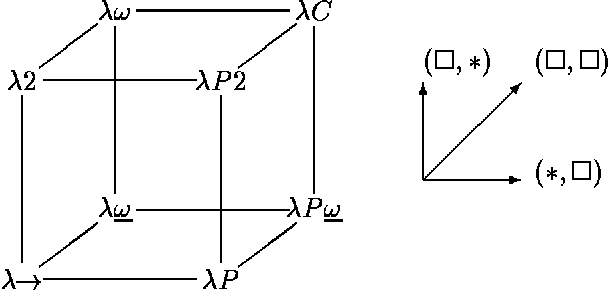
\includegraphics[scale=0.3]{lection-00-cube.png}}
\end{center}
Типовые системы и языки программирования:

Классические и функциональные языки:

\begin{tabular}{lll}
$\lambda_\rightarrow$          & Классический Паскаль\\
$\lambda_{\underline{\omega}}$ & Система F\\
$\lambda_\omega$& Haskell, Ocaml
\end{tabular}

\vspace{0.3cm}
Языки с зависимыми типами данных (обычно около $\lambda C$):\\
Idris, Coq, Agda, Arend, C++ :).
\end{frame}

\begin{frame}{$(\Leftarrow)$: изучение логики и доказательств через написание программ}
\begin{itemize}
\item Пер Мартин-Лёф, Intuonistic Type Theory: версии 1972 и 1979.
\item Множество расширений и вариантов.
\item Такие инструменты как Coq, Agda, Lean используют варианты этой теории.
\item Мы будем рассматривать некоторую родственную теорию, гомотопическую теорию типов.
\end{itemize}
\end{frame}


\begin{frame}[fragile]{Гомотопическая теория типов}
Владимир Александрович Воеводский, 1966-2017. \vspace{0.5cm}

... Математика находится на пороге кризиса, а точнее двух кризисов. Первый связан с отрывом 
математики <<чистой>> от математики прикладной. Понятно, что рано или поздно встанет вопрос о 
том, а почему общество должно платить деньги людям, которые занимаются вещами, не имеющими 
никаких практических приложений. Второй, менее очевидный, связан с усложнением чистой математики, 
которое ведет к тому, что, опять же рано или поздно, статьи станут слишком сложными для детальной 
проверки и начнется процесс накопления незамеченных ошибок ...

\end{frame}

\begin{frame}[fragile]{Гомотопическая теория типов}
\begin{itemize}
\item Центральный вопрос --- что такое равенство.
\item Классический матлог: это предикат, удовлетворяющий свойствам.
\item Однако, свойства обычно слишком общие (класс эквивалентности?). Интуитивно хочется большего,
равенство не всегда просто эквивалентность.
\item Изоморфизм Карри-Ховарда-Воеводского:
\begin{tabular}{lll}
Логика & $\lambda$-исчисление & Топология\\\hline
Утверждение & Тип & Пространство \\
Доказательство & Значение & Точка в пространстве\\
Предикат $(=)$ & Зависимый тип $(=)$ & Путь между точками
\end{tabular}
\item Реализация: кубическая теория типов, Аренд.
\end{itemize}
\end{frame}

\begin{frame}{Чем естественно такое определение равенства?}
\begin{multicols}{2}
Целые числа --- класс эквивалентности пар $\langle a,b\rangle$ при $a,b\in\mathbb{N}_0$, понимаемых как $a-b$.

Точнее:
$\langle a,b\rangle\approx\langle c,d\rangle := a+d = b +c$
$\mathbb{Z} := \{\langle a,b\rangle\ |\ a,b\in\mathbb{N}_0\}/_\approx$


Рассмотрим топологическое пространство с носителем $Z = \{\langle a,b\rangle\ |\ a,b\in\mathbb{N}_0\}$,\\
открытыми множествами назовём все диагональные прямые $x = y + c$ и $y = x + c$.\\

\columnbreak


\tikz{
   \draw[thick=2,-stealth] (0,-0.5) -- (0,4.5);
   \draw[thick=2,-stealth] (-0.5,0) -- (4.5,0);

   \foreach \t in {0,...,4}
   {
      \draw[thick=3,color=red] (\t,0) -- (4,{4-\t});
      \draw[thick=3,color=red] (0,\t) -- ({4-\t},4);
   }

   \foreach \x in {0,...,4}
   \foreach \y in {0,...,4}
   {
      \node[shape=circle, fill=black, scale=0.3] (\x-\y) at (\x,\y) {};
   }
}

$\langle a,b \rangle = \langle c,d\rangle$ эквивалентно существованию пути
$\pi : [0,1] \rightarrow Z$, что $\pi(0) = \langle a,b\rangle$ и $\pi(1) = \langle c,d\rangle$.


\end{multicols}
\end{frame}

\begin{frame}{Построение курса}
\begin{enumerate}
\item Аналогично с матлогом, будет разделение на теорию и практику.
\item Теория: знание определений, идей, теорем.
\item Практика: лабы на доказательства теорем с использованием языка Аренд, возможны дополнительные околокомпиляторные лабы.
\item Для закрытия предмета надо набрать баллы практическими заданиями и сдать зачёт/экзамен.
\end{enumerate}
\end{frame}

\end{document}
